%%%%%%%%%%%%%%%%%%%%%%%%%%%%%%%%%%%%%%%%%
% FRI Data Science_report LaTeX Template
% Version 1.0 (28/1/2020)
% 
% Jure Demšar (jure.demsar@fri.uni-lj.si)
%
% Based on MicromouseSymp article template by:
% Mathias Legrand (legrand.mathias@gmail.com) 
% With extensive modifications by:
% Antonio Valente (antonio.luis.valente@gmail.com)
%
% License:
% CC BY-NC-SA 3.0 (http://creativecommons.org/licenses/by-nc-sa/3.0/)
%
%%%%%%%%%%%%%%%%%%%%%%%%%%%%%%%%%%%%%%%%%


%----------------------------------------------------------------------------------------
%	PACKAGES AND OTHER DOCUMENT CONFIGURATIONS
%----------------------------------------------------------------------------------------
\documentclass[fleqn,moreauthors,10pt]{ds_report}
\usepackage[english]{babel}
\usepackage{csquotes}
\usepackage{tcolorbox}
\usepackage{calc}
\usepackage{booktabs}


\newsavebox\mybox
\newenvironment{aquote}[1]
  {\savebox\mybox{#1}\begin{quote}\openautoquote\hspace*{-.7ex}}
  {\unskip\closeautoquote\vspace*{1mm}\signed{\usebox\mybox}\end{quote}}

\graphicspath{{fig/}}


\newtcbox{\labelbox}[1][red]{on line,
arc=0pt,outer arc=0pt,colback=#1!10!white,colframe=#1!50!black,
boxsep=0pt,left=1pt,right=1pt,top=1pt,bottom=0.8pt,
boxrule=0pt,bottomrule=0.6pt,toprule=0.6pt,width=5cm}

\newcommand\bm{0.2pt}


%----------------------------------------------------------------------------------------
%	ARTICLE INFORMATION
%----------------------------------------------------------------------------------------

% Header
\JournalInfo{FRI Natural language processing course 2021}

% Interim or final report
\Archive{Project report} 
%\Archive{Final report} 

% Article title
\PaperTitle{Offensive language exploratory analysis} 

% Authors (student competitors) and their info
\Authors{Maša Kljun, Matija Teršek}

% Advisors
\affiliation{\textit{Advisors: Slavko Žitnik}}

% Keywords
\Keywords{Hate speech, TF-IDF, embeddings, exploratory analysis, NLP ...}
\newcommand{\keywordname}{Keywords}


%----------------------------------------------------------------------------------------
%	ABSTRACT
%----------------------------------------------------------------------------------------

\Abstract{
In this paper we focus on the exploratory analysis of 10 different subgroups of hate speech. We use natural language processing techniques in order to find the underlying structure and connections/relations between the subgroups. We focus on data extracted from Twitter and online forums. First we use classic approaches, such as TF-IDF, BoW, and LDA, then we move on to more sophisticated methods such as embeddings. \textcolor{blue}{Note to professor: More to come in the next submission.}
}

%----------------------------------------------------------------------------------------

\begin{document}

% Makes all text pages the same height
\flushbottom 

% Print the title and abstract box
\maketitle 

% Removes page numbering from the first page
\thispagestyle{empty} 

%----------------------------------------------------------------------------------------
%	ARTICLE CONTENTS
%----------------------------------------------------------------------------------------

\section*{Introduction}
In the last few years social media grew exponentially and with it also the ability of people to express themselves online. By enabling people to write on different online platforms without even identifying themselves it lead to a new era of freedom of speech. As this new medium for communication and writing brought many positive things, it also has its downside. Social media has become a place where heated discussions happen and often result in insults and hatred. It is an important task to recognize hate speech and to prevent it.

Hate speech is defined as \textit{abusive or threatening speech or writing that expresses prejudice against a particular group, especially on the basis of race, religion, or sexual orientation}\cite{hate_speech}. We can see that the definiton is very vague. Having said that, the goal of our paper is to help distinguish different types of hate speech and find the specific keywords of its subgroups in order to explain its structure. This could help with its identification and classification. In this paper we focus on ten subgroups of hate speech - \textit{abusive, hateful, spam, general hate speech, profane, offensive, cyberbullying, racism, sexism, } and \textit{benevolent sexism}. With understanding the structure of these groups, the goal is to also find similarities and connections between them.

There has been done a lot of research regarding the hate speech, however these works are usually focused on the classification of hate speech. One of the first works include \cite{spertus1997smokey} who built the decision tree based classifier Smokey for abusive message recogniton and classification. Some other works that focus mainly on classification include \cite{waseem2016you} who compare the classification accuracy of models trained on expert and amateur annotations, \cite{gamback2017using} who use convolutional neural networks for classification into four predefined categories, and \cite{martins2018hate} who use different natural language processing techniques for expanding datasets with emotional information for better classification. In the last years, especially deep learning models are often used for detection and classification of hate speech, such as \cite{rizoiu2019transfer} who propose a sophisticated method that is a combination of a deep neural network architecture with transfer learning.
There is a also a lot of related work that focuses on creating large datasets such as \cite{chung2019conan} who create a large-scale, multilingual, expert based dataset of hate speech. 

What is less common in the research area of hate speech is analysis of relationships between different types of hate speech and the importance of specific keywords. Some examples include \cite{xu2012learning}, who try to separate bullying from other social media posts and try to discover topic of bullying using topic modeling with Latent Dirichlet Allocation (LDA). \cite{calderon2020topic} model hate speech against immigrants on Twitter in Spain. They try to find underlying topic of hate speech using LDA, discovering features of different dimensions of hatespeech, including foul language, humiliation, irony, etc. \cite{schmidt2017survey} conduct a survey about hate speech detection and describe key areas that have been explored, regarding the topic modeling, as well as sentiment analysis.

\textcolor{blue}{Note to professor: Our goal for the future is first a deeper analysis of the obtained data. We will try to extract some underlying topics for each label and present the main findings (LDA). Use TF-IDF to find the most common $n$-grams for each label. And in the future focus on the newer approaches, such as embedding with the further goal of exploring the relationships between types of hate speech. We hope that we can determine a more precise plan on the first submission defense.}

\textcolor{gray}{This paper is organized as follows: TODO at the end of the report}

% --------------------------------------------------------------------------------------------------------------------------------

\section*{Data}

We use six publicly available datasets for our exploratory analysis. We combine datasets \cite{waseem2016you}, \cite{rizoiu2019transfer}, and \cite{jha2017does} into one large dataset (reffered to as Dataset SRB) as they include same categories of hate speech. We make labels \textit{sexism}, \textit{racism}, and \textit{both} from \cite{waseem2016you} and \cite{rizoiu2019transfer}. The third dataset (\cite{jha2017does}) that we use contains label \textit{hostile sexism}, where marked tweets are already included in the first two datasets under \textit{sexism}, and label \textit{benevolent sexism}, which we rename to \textit{benevolent}. We obtain a dataset with $6069$ samples that are labeled either $sexism$, $racism$, $both$, or $benevolent$.
The fourth dataset (reffered to as Dataset AHS)\cite{founta2018large} that we use has $3$ categories - \textit{abusive,
hateful, spam}. As this is the original dataset no additional merging is needed. We obtain a dataset with $13776$ tweets with the mentioned labels. Note that we exclude \textit{None} label from both datasets, as we do not need it for the analysis.
We show the distribution of individual categories from datasets SRB and AHS in Figures \ref{fig:distribution_tweets_dataset1} and \ref{fig:distribution_tweets_dataset2}, respectively. Note that the numbers of samples might not match the numbers in the original papers, due to the Twitter removing the tweets, making them unavailable for us to analyze. We also provide an example for each label.

\begin{tcolorbox}[colback=black!8,width=0.9\linewidth, center,arc=8pt,sharp corners=downhill, boxrule=0.3pt, left=\bm, top=\bm, right=\bm, bottom=\bm, fontupper=\small]
\labelbox{\textit{Racism}} - "He can't be a server at our restaurant, that beard makes him look like a terrorist." Everyone laughs. \#fuckthanksgiving
\end{tcolorbox}

\begin{tcolorbox}[colback=black!8, width=0.9\linewidth, center,arc=8pt,sharp corners=downhill, boxrule=0.3pt, left=\bm, top=\bm, right=\bm, bottom=\bm, fontupper=\small]
\labelbox{\textit{Sexism}} - \#katieandnikki stop calling yourselves pretty and hot..you're not and saying it a million times doesn't make you either...STFU
\end{tcolorbox}

\begin{tcolorbox}[colback=black!8, width=0.9\linewidth, center,arc=8pt,sharp corners=downhill, boxrule=0.3pt, left=\bm, top=\bm, right=\bm, bottom=\bm, fontupper=\small]
\labelbox{\textit{Benevolent}} - It's "NEXT to every successful man, there's a woman"
\end{tcolorbox}

\begin{tcolorbox}[width=0.9\linewidth, center,arc=8pt,sharp corners=downhill, boxrule=0.3pt, left=\bm, top=\bm, right=\bm, bottom=\bm, fontupper=\small]
\labelbox{\textit{Spam}} - RT @OnlyLookAtMino: [!!] \#WINNER trending \#1 on melon search
\end{tcolorbox}

\begin{tcolorbox}[width=0.9\linewidth, center,arc=8pt,sharp corners=downhill, boxrule=0.3pt, left=\bm, top=\bm, right=\bm, bottom=\bm, fontupper=\small]
\labelbox{\textit{Abusive}} - You Worried About Somebody Bein Ugly... Bitch You Ugly...
\end{tcolorbox}

\begin{tcolorbox}[width=0.9\linewidth, center,arc=8pt,sharp corners=downhill, boxrule=0.3pt, left=\bm, top=\bm, right=\bm, bottom=\bm, fontupper=\small]
\labelbox{\textit{Hateful}} - i hope leaders just kick retards that fake leave teams today
\end{tcolorbox}

\begin{figure}[ht]\centering
	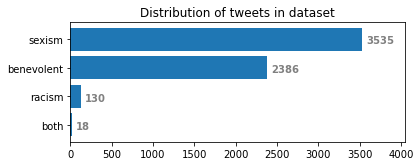
\includegraphics[width=\linewidth]{distribution_tweets_dataset1.png}
	\caption{\textbf{Distribution of tweets in SRB dataset.} This figure shows the distribution of hate speech categories in the SRB dataset. We can see that \textit{sexism} and \textit{benevolent} are well represented, whereas \textit{racism} and \textit{both} are far less frequent. Original set contains more tweets labeled \textit{racism}, but due to their removal we cannot obtain them.}
	\label{fig:distribution_tweets_dataset1}
\end{figure}

\begin{figure}[ht]\centering
	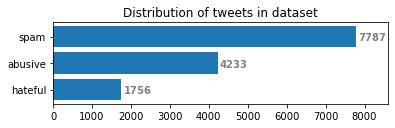
\includegraphics[width=\linewidth]{distribution_tweets_dataset2.png}
	\caption{\textbf{Distribution of tweets in AHS dataset.} We see that the \textit{spam} is the most represented label in the dataset, which represents the majority of the dataset. This is followed by the \textit{abusive} tweets and there is the least \textit{hateful} tweets. We can see that categories in this dataset are well represented.}
	\label{fig:distribution_tweets_dataset2}
\end{figure}

\noindent Additionally we use the dataset of comments extracted from the League of Legends community \cite{bretschneider2016detecting}. We preprocess the dataset given in the SQL format to a more readable CSV form and keep only the posts that are annotated as harassment. We obtain $259$ examples of cyberbullying examples. The sixth dataset that we use was designed for the problem of the hate speech identification and classification, but we use the labels from the train and test set and merge them into one big dataset that we use for our analysis. It provides tags of \textit{hatespeech, profane}, and \textit{offensive}, so we refer to the dataset as HPO. It consists of 2549 tweets, distribution of which can be seen in Figure \ref{fig:distribution_tweets_hpo}. We again provide an example for each of the labels.

\begin{tcolorbox}[colback=black!8, width=0.9\linewidth, center,arc=8pt,sharp corners=downhill, boxrule=0.3pt, left=\bm, top=\bm, right=\bm, bottom=\bm, fontupper=\small]
\labelbox{\textit{Cyberbullying}} - plot twist she's a fggt
\end{tcolorbox}

\begin{tcolorbox}[width=0.9\linewidth, center,arc=8pt,sharp corners=downhill, boxrule=0.3pt, left=\bm, top=\bm, right=\bm, bottom=\bm, fontupper=\small]
\labelbox{\textit{Hatespeech}} - Johnson you liar. You don't give a flying one for the Irish
\end{tcolorbox}

\begin{tcolorbox}[width=0.9\linewidth, center,arc=8pt,sharp corners=downhill, boxrule=0.3pt, left=\bm, top=\bm, right=\bm, bottom=\bm, fontupper=\small]
\labelbox{\textit{Offensive}} - \#FuckTrump And retired porn star Melania too.
\end{tcolorbox}

\begin{tcolorbox}[width=0.9\linewidth, center,arc=8pt,sharp corners=downhill, boxrule=0.3pt, left=\bm, top=\bm, right=\bm, bottom=\bm, fontupper=\small]
\labelbox{\textit{Profane}} - Fuck Trump and anybody who voted for that Lyin POS!  \#FuckTrump
\end{tcolorbox}

\begin{figure}[ht]\centering
	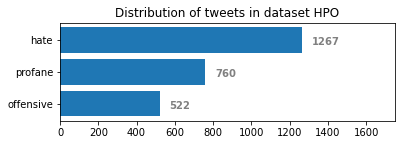
\includegraphics[width=\linewidth]{distribution_tweets_hpo.png}
	\caption{\textbf{Distribution of tweets in HPO dataset.} The most used label is \textit{hatespeech}. It is followed by \textit{profane} and then \textit{offensive}, which have a similar number of tweets.}
	\label{fig:distribution_tweets_hpo}
\end{figure}

\noindent We also use the dataset of Wikipedia comments \cite{dixon2017ex}, that are marked as either \textit{toxic}, \textit{sever toxic}, \textit{obscene}, \textit{identity hate}, \textit{threat}, and \textit{insult}. We merge the first two categories into \textit{toxic}. It is important to note that each comment in this dataset might have multiple labels, so the results for those tags might be similar. Original dataset contains $159571$ tweets, $16225$ of which are labeled. We show the distribution of the labels in Figure \ref{fig:distribution_wiki_dataset}. We denote this dataset as TOITI in the future text.

\begin{tcolorbox}[width=0.9\linewidth, center,arc=8pt,sharp corners=downhill, boxrule=0.3pt, left=\bm, top=\bm, right=\bm, bottom=\bm, fontupper=\small]
\labelbox{\textit{Threat}} - SHUT UP, YOU FAT POOP, OR I WILL KICK YOUR ASS!!!
\end{tcolorbox}

\begin{tcolorbox}[width=0.9\linewidth, center,arc=8pt,sharp corners=downhill, boxrule=0.3pt, left=\bm, top=\bm, right=\bm, bottom=\bm, fontupper=\small]
\labelbox{\textit{Obscene}} - you are a stupid fuck and your mother's cunt stinks
\end{tcolorbox}

\begin{tcolorbox}[width=0.9\linewidth, center,arc=8pt,sharp corners=downhill, boxrule=0.3pt, left=\bm, top=\bm, right=\bm, bottom=\bm, fontupper=\small]
\labelbox{\textit{Insult}} - Fuck you, block me, you faggot pussy!
\end{tcolorbox}

\begin{tcolorbox}[width=0.9\linewidth, center,arc=8pt,sharp corners=downhill, boxrule=0.3pt, left=\bm, top=\bm, right=\bm, bottom=\bm, fontupper=\small]
\labelbox{\textit{Toxic}} - What a motherfucking piece of crap those fuckheads for blocking us!
\end{tcolorbox}

\begin{tcolorbox}[width=0.9\linewidth, center,arc=8pt,sharp corners=downhill, boxrule=0.3pt, left=\bm, top=\bm, right=\bm, bottom=\bm, fontupper=\small]
\labelbox{\textit{Identity}} - A pair of jew-hating weiner nazi schmucks.
\end{tcolorbox}


\begin{figure}
	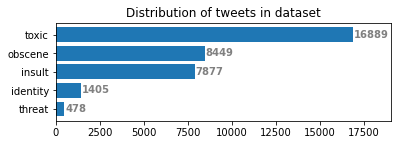
\includegraphics[width=\linewidth]{distribution_wiki_dataset.png}
	\caption{\textbf{Distribution of tweets in TOITI}. We see that most of the comments are labeled as \textit{toxic}. Around half of them are \textit{obscene} and around half are also labeled as \textit{insult}. \textit{Identity hate} and \textit{threat} are far more uncommon in this dataset.}
	\label{fig:distribution_wiki_dataset}
\end{figure}

\section*{Data preprocessing}
Before applying any methods we first preprocess all of our data. We separate datasets into subgroups only, where each contains multiple documents - tweets belonging to this category. We remove retweet text RT, hyperlinks, hashtags, taggings, new lines, and zero length tweets. We further filter out tokens that not contain letters, e.g., raw punctuation.

% --------------------------------------------------------------------------------------------------------------------------------
\section*{Methodology}
We start the analysis with more traditional approaches, and continue with neural approaches.

% --------------------------------------------------------------
\subsection*{LDA}
We use Latent Dirchilet Allocation (LDA) in combination with Bag-of-Words (BoW) and TF-IDF in hopes of finding obvious topics from all the provided comments / tweets. We try to determine 15 different topics, which is the same as the number of labels we have in our datasets. Results using BoW and TF-IDF are similar, however, we cannot clearly distinguish between the topics and connect obtained topics to the existing labels, aside from one topic, which is related to sexism. Top 5 most related words are: \textit{penis, rape, image, live, vagina}.

% --------------------------------------------------------------
\subsection*{TF-IDF}
We continue with the analysis of datasets with a traditional method TF-IDF as we want to see the most relevant words for each category of offensive language that we have in the dataset. We show the results in Table \ref{tab:tf-idf}. We can see that some of the categories have similar unigrams that achieved the highest TF-IDF score. An example of categories with the same highest scored unigrams are \textit{insult} and \textit{obscene}. This makes it harder to differentiate between the categories. It is important to note, that such examples might also occur due to subjective labeling in the provided datasets, as well as people not clearly differentiating between these categories. Most datasets are not labeled by experts, but with the help of platforms such as FigureEight or Amazon Mechanical Turk. From the results in Table \ref{tab:tf-idf}, we could assume that most people perceive categories such as \textit{insult} and \textit{obscene} or \textit{threat} and \textit{toxic} similarly. On the other hand, categories such as \textit{spam} or \textit{cyberbullying} are clearly differentiable from other categories. We can also see a lot of categories including Trump related words (\textit{hatespeech, profane}, and \textit{offensive}). Those categories are taken from the same dataset, and we can see that such labels will contain words that are related. So the words connected to those labels might also be connected to some bigger topic, which depends on the annotator's choice from where to extract the tweets / comments.

\begin{table}[htb]
\scriptsize
\centering
\begin{tabular}{l|l}
\toprule
\textbf{category}   & \textbf{unigrams with highest TF-IDF score} \\ \midrule
racism     & peopl, white, terror, man, look                \\ \hline
sexism     & feminazi, women, think, sexist, notsexist                \\ \hline
benevolent & women, classi, sassi, nasti, gonna            \\ \hline
abusive    & know, stupid, shit, like, idiot  \\ \hline
hateful    & peopl, trump, nigga, like, idiot    \\ \hline
spam       & giveaway, game, enter, work, home            \\ \hline
cyberbullying       & one, guy, good, gone, go             \\ \hline
hatespeech      & world, trumpisatraitor, trump, shameonicc, peopl             \\ \hline
identity hate       & fuck, shit, littl, like, one             \\ \hline
insult       & delet, go, ass, stupid, bitch        \\ \hline
obscene       & delet, go, stupid, bitch, ass             \\ \hline
offensive       & trumpisatraitor, like, douchebag, fucktrump, get            \\ \hline
profane       & trump, shit, say, resist, peopl             \\ \hline
threat       & fuck, get, die, want, find           \\ \hline
toxic       & fuck, get, bitch, want, block             \\ \bottomrule
\end{tabular}
\caption{Table shows 5 highest scoring unigrams for each label we investigate. We choose the parameters, which we believe provide us the most meaningful unigrams, so we consider words that appear in at least $5\%$ and less than $60\%$ of the documents.}
\label{tab:tf-idf}
\end{table}
% --------------------------------------------------------------
\subsection*{Non-contextual word embeddings}
First we select top 3 unigrams from TF-IDF results in the previous subsection (if available in the model) and find 20 most similar embeddings of pre-fitted Word2Vec and GloVe (FastText unfortunatelly does not run due to available computational resources). We visualize the results with the help of t-SNE. We show the results in \ref{fig:embedding_words}. From both plots we can see that words (and its neighbors) like bitch, ass, nigga, shit, fuck, idiot, stupid, and docuhebag are relatively closely together. This could indicate a relation between \textit{abusive, hateful, insult, obscene, identity hate}, and \textit{toxic}. We can also see that classy, nasty, sassy, feminazi, and sexist are closely related - sometimes some words are more related in Word2Vec than in Glove and vice versa. From this we can see a relation between \textit{sexism} and \textit{benevolent sexism}, which is expected as they are correlated. Relationships between certain words can also vastly differ in Word2Vec and Glove. For example giveaway and game are relatively close in Word2Vec, but are further apart in Glove. Similarly, terror and white (both common unigrams of \textit{racism} label) are far away in Word2Vec, but close in Glove. However, terror stands out from other words in both embeddings, which might indicate that racism is at least in some way different to other labels. Similarly, words from \textit{spam} are usually more separated from words of other labels, also indicating another more clearly distinguishable group. Trump is relatively close to a lot of words in Word2Vec - women, world, peopl, sexist, die, little, guy. This could imply that general \textit{hatespeech} and \textit{hateful} are connected to \textit{sexism, identity hate, threat} and also \textit{cyberbullying}. 

\begin{figure*}[ht]\centering
	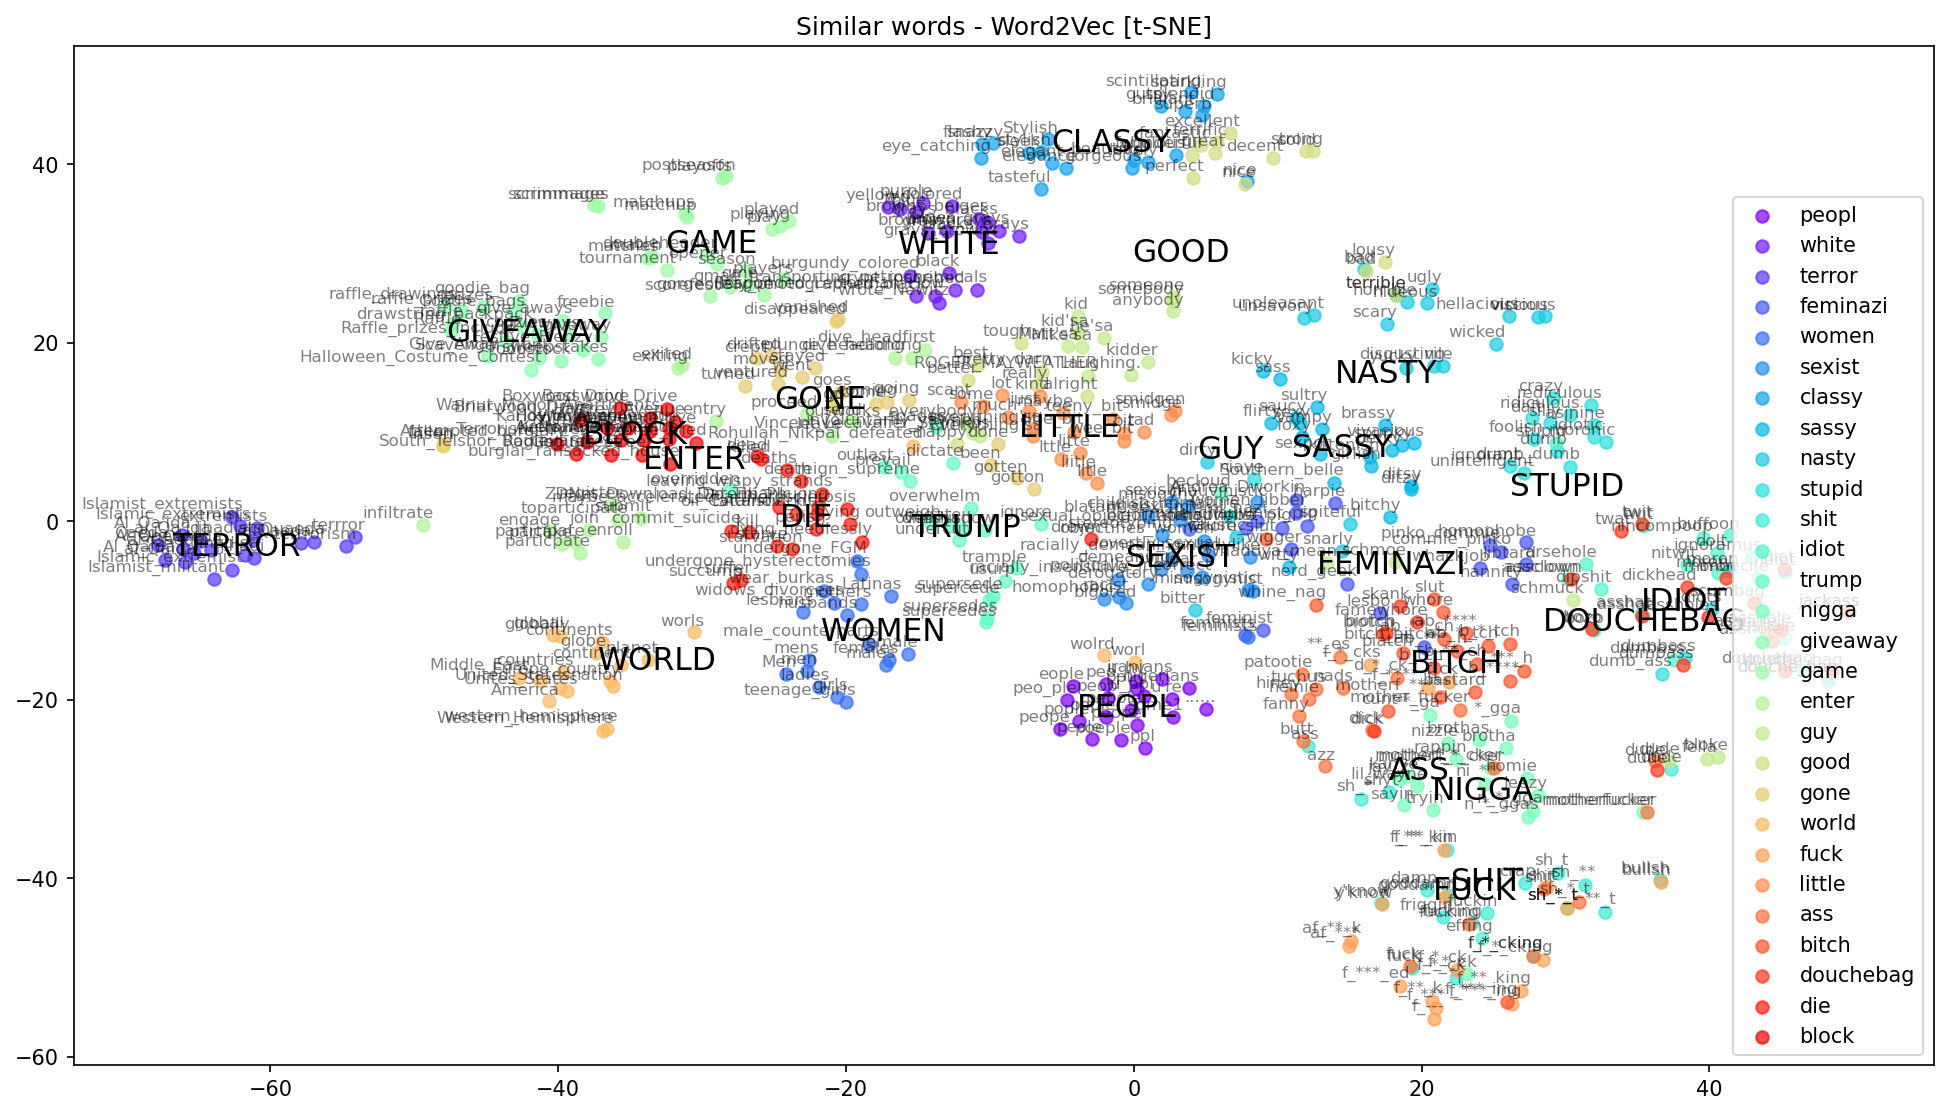
\includegraphics[width=0.495\linewidth]{SimilarWords - word2vec - t-SNE.png}
	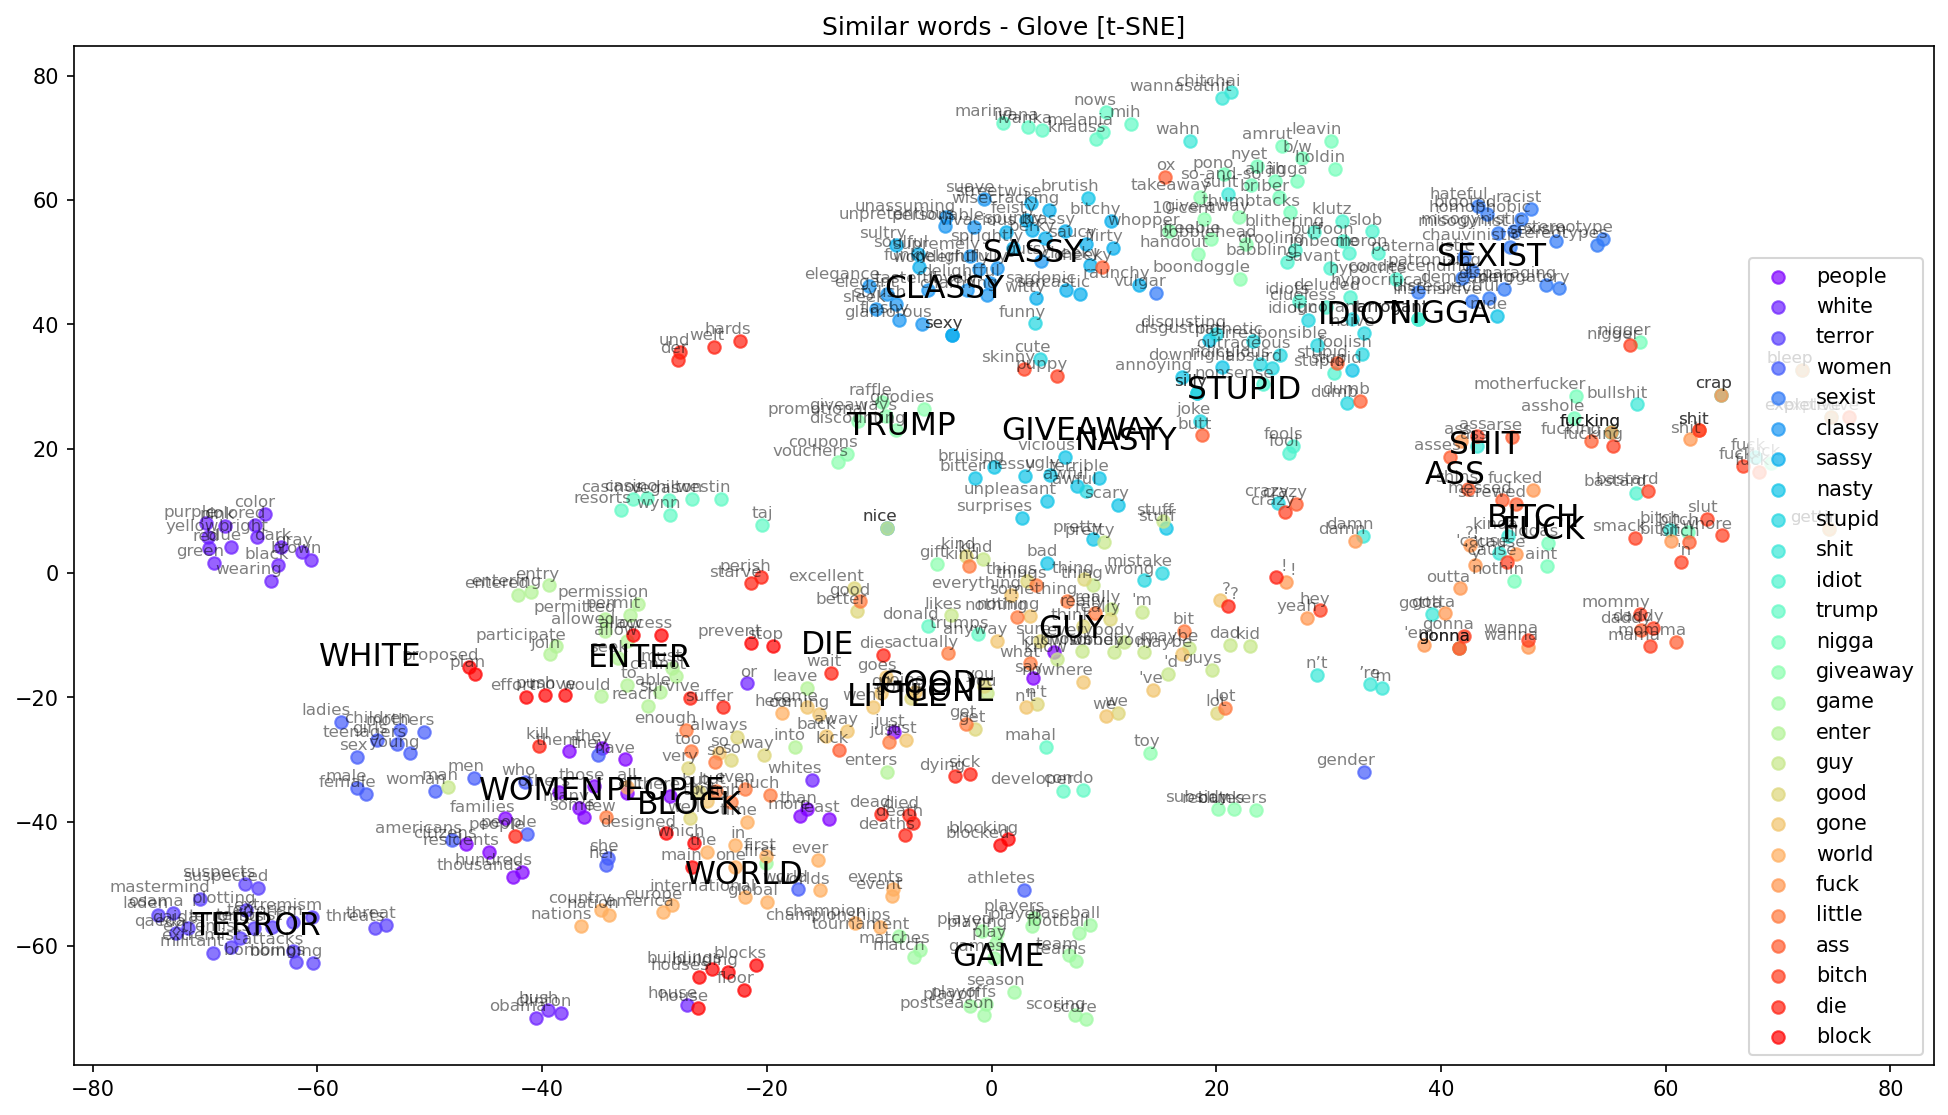
\includegraphics[width=0.495\linewidth]{SimilarWords - Glove - t-SNE.png}
	\caption{\textbf{Word2Vec and Glove similar words.} Left figure shows Word2Vec embeddings of neigbouring words of top unigrams from Table \ref{tab:tf-idf} and the right figure shows Glove embeddings.}
	\label{fig:embedding_words}
\end{figure*}

Additionally, after finding some initial relations with previous approaches, we also find most similar words to the category labels and compare them in a similar fashion.

\section*{Discussion}

Use the Discussion section to objectively evaluate your work, do not just put praise on everything you did, be critical and exposes flaws and weaknesses of your solution. You can also explain what you would do differently if you would be able to start again and what upgrades could be done on the project in the future.


%----------------------------------------------------------------------------------------
%	REFERENCE LIST
%----------------------------------------------------------------------------------------
\bibliographystyle{unsrt}
\bibliography{report}


\end{document}